\documentclass[10pt]{article}

% Idioma y codificación
\usepackage[utf8]{inputenc}
\usepackage[spanish]{babel}

% Márgenes
\usepackage{geometry}
\geometry{top=2.5cm, bottom=2.5cm, left=2.5cm, right=2.5cm}

% Gráficos
\usepackage{graphicx}
\usepackage{graphics}
\usepackage{wrapfig}
\usepackage{pdfpages}
\usepackage{multicol}
\usepackage{float}
\usepackage{titling}

% Listings para código
\usepackage{listings}
\usepackage{xcolor}
\usepackage{caption}
\usepackage{capt-of}
\usepackage{titling}
\lstdefinestyle{terminal}{
	backgroundcolor=\color{gray!10},
	basicstyle=\ttfamily\small,
	keywordstyle=\color{blue},
	commentstyle=\color{gray},
	frame=single,
	columns=fullflexible,
	morecomment=[l]{//}
}

\usepackage{booktabs}
\usepackage{tabularx}
\usepackage{comment}

\usepackage{listings}
\lstset{
	inputencoding=utf8,
	extendedchars=true,
	literate={á}{{\'a}}1 {é}{{\'e}}1 {í}{{\'i}}1 {ó}{{\'o}}1 {ú}{{\'u}}1 {ñ}{{\~n}}1
}

% Hipervínculos
\usepackage[hidelinks]{hyperref}
\hypersetup{
	colorlinks=true,
	linkcolor=blue,
	filecolor=magenta,
	urlcolor=cyan,
}

% Encabezados y pies de página
\usepackage{fancyhdr}
\pagestyle{fancy}
\fancyhf{}
\fancyfoot[R]{\thepage}
\usepackage{subcaption}

% Formato de títulos
\usepackage{titlesec}
\titleformat{\subsection}{\normalfont\large\bfseries}{\hspace{1em}\thesubsection}{1em}{}
\titleformat{\subsubsection}{\normalfont\normalsize\bfseries}{\hspace{2em}\thesubsubsection}{1em}{}

% Datos de la portada
\title{
	\textit{CARD PARTNER}\\
	Una web para amantes de los \textit{TCGS}}


\author{
	\textbf{\small ALVAREZ FULCONIS, MARCOS PALATINO}\\
	\textbf{\small LOPEZ PRIMO, ALVARO}\\
	\textbf{\small OTERO GARCIA, SERGIO}\\
	\textbf{\small SANTIESTEBAN MENDO, EDGAR}}

\date{Curso 25-26}

\makeatletter
\let\thetitle\@title
\let\theauthor\@author
\let\thedate\@date
\makeatother

\begin{document}
	
	\begin{titlepage}
		\centering
		
\includegraphics[scale=0.3]{./Recursos/UVA-3881270087.pdf}\\[0.5cm]
		\rule{\linewidth}{0.2mm}\\[0.4cm]
		{\huge\bfseries \thetitle\par}
		\rule{\linewidth}{0.2mm}\\[1.5cm]
		{\Large\bfseries Servicios y Sistemas Web}\\[0.3cm]
		{\large\bfseries Laboratorio L2 \\ GRUPO 33}\\[1cm]
		{\Large \theauthor}\\[1.5cm]
		{\Large \thedate}
	\end{titlepage}
	
	\pagenumbering{gobble}
	
	\renewcommand{\contentsname}{Índice}
	\tableofcontents \newpage
	
	\pagenumbering{arabic} % reinicia la numeración en números arábigos
	\setcounter{page}{1}   % empieza desde la página 1
	
	\section{Descripción del problema}
	Los \textit{\textbf{TCG}} (\textit{Trading Card Games}) están en auge y mucha gente necesita una manera de poder iniciarse en un mundo tan complejo.\\
	Debido a su gran catidad, variedad de  mazos, y \textit{META}s (\textit{Most Efficience Tactiques Avaliable}) los jugadores necesitan una herramienta para  consultar resultados de competiciones, mazos, compartir los que hayan creado y enterarse de que cartas están \textit{banned} (prohibidas) en los torneos oficiales\ldots \\ 
	
	Para esto hemos decidido crear una web donde se podrán realizar la siguientes tareas:
	\begin{multicols}{2} 
		\begin{itemize}
			\item Crear cuentas de usuario
			\begin{itemize} 
				\item Cuenta con correo y contraseña
				\item Cambio de contraseña
				\item Subida de mazos creados
				\item Listado de mazos creados
				\item Lista de mazos guardados
				\item Permitir comentarios y valoraciones en mazos
			\end{itemize}
			
			\item Creador de mazos
			\item Novedades del TCG
			\item Listado de mazos
			\begin{itemize}
				\item Por Líder
				\item Por expansión
			\end{itemize}
			
			\item Estadísticas de los mazos
			\item Vista para ver todas las cartas
			\begin{itemize}
				\item Por expansión
				\item Por color
			\end{itemize}
			
			\item Listado de torneos (ganadores/mazos)
			\item Guía básica del juego
			\begin{itemize}
				\item Explicación de normas
				\item Mazos para principiantes
			\end{itemize}
			
			\item Selector de idioma
			\item Consultar precios de cada carta
			\item Usuario admin
		\end{itemize}
	\end{multicols} 
	Permitiendo en primer lugar tener una web de referencia para iniciarse en cada uno de los \textit{TCGs}, conocer a la comunidad, torneos, tiendas locales y en segundo lugar para  facilitar la creación de los mazos, permitir a otros usuarios comentar modificaciones, así como tener un lugar donde poder consultar todas las cartas con su precio en caso de querer comprarse las mismas.\\
	Debido a la gran variedad de \textit{TCGs}, vamos a usar el de \textit{One Piece} como referencia. \\
	Actualmente los usuarios, emplean 3 webs para las tareas antes mencionadas:
	\begin{enumerate}
		\item \href{https://www.cardmarket.com/es/OnePiece}{\textit{Card Market}}: El sitio más popular de compra venta de cartas de múltiples \textit{TCGs}.
		\item \href{https://deckbuilder.egmanevents.com/optcg/cards}{\textit{EggmanEvents}}: El lugar más popular para consultar mazos, carga muy lenta, con una experiencia no centrada en el usuario novato, sin la posiblidad de crear tus propios mazos, sino emplear ya mazos empleados en torneos.
		\item \href{https://en.onepiece-cardgame.com/beginners/}{\textit{One Piece Card Game}}:El sitio oficial del juego de cartas donde se pueden encontrar manuales o \textit{quick start guides} sobre como empezar a jugar así como una lista de todos los productos lanzados en este \textit{TCG}.
		\item \href{https://onepiece.limitlesstcg.com}{\textit{One Piece Limitless}}: REVISAR ESTE, Torneos y estadisticas, meta, creador de mazos, cartas y simulador del juego.
	\end{enumerate}
	Nuestra idea es unificar estas webs en una sóla, que coja el esqueleto de \textit{Eggman}, integre una diseño más centrado en el usuario con la posibilidad de consultar el precio de cada una de las cartas y del total de un mazo así como tener una sección para jugadores novatos donde se les de una explicación del juego y unas recomendaciones de por dónde empezar.
	
	%• La descripción debe ser breve y concisa y limitarse a las metas de alto nivel del proyecto.
	%• El problema se describirá en términos de tareas o funcionalidades de alto nivel que
	%pueden realizar los usuarios y de los posibles contextos en que las tareas podrán tener
	%lugar.
	%• Se describirá qué aspectos de las tareas se mejorarán con la solución técnica propuesta.
	%• Se describirá el contexto del problema de forma que mejore la comprensión y alcance del proyecto.
	%• Se discutirán posibles soluciones existentes.
	
	\newpage
	\section{Usuarios objetivo}
	En esta parte, comentaremos para quienes va destinada nuestra web, dividiéndolos en dos grupos; usuarios novatos y experimentados, en función del conocimiento que tengan en el juego.
	
	El primero de ellos, los novatos, son personas que sienten curiosidad por el juego de cartas, quizás porque se basa en una serie que les gusta o porque un conocido se lo ha recomendado, pero no tienen experiencia previa con el juego. Para ellos, se creará una sección de la web donde podrán entender el funcionamiento básico del juego, así como una sección de recomendaciones de qué mazos son más simples para poder iniciarse en el juego de cartas.\\
	
	El segundo son los jugadores experimentados, los cuales ya conocen las mecánicas del \textit{TCG} y buscan mazos \textit{META} o probar combinaciones de cartas así como compartir dichos mazos con el resto de los jugadores y dar consejos sobre mazos que han sido compartidos. Su objetivo es mantenerse en la escena competitiva, y fomentar la comunidad del propio \textit{TCG}
	%• El grupo de usuarios a que se destine el sitio web debe ser sensato y no trivial.
	%• Se describirá el grupo de usuarios con suficiente detalle como para poder diferenciarlo de otros.
	%• Se describirán las necesidades y expectativas reconocidas en el grupo de usuarios objetivo.
	
	
	\section{Borrador de solución}
	%\begin{itemize}
	%\item Se conjugará texto y bocetos (escritos a mano y escaneados si resulta más cómodo) para
	%describir de forma general la solución propuesta.
	%\item Se valorará claridad, generalidad y adecuación de la solución inicial propuesta.
	%\end{itemize}
	
	
	\subsection{Primer versión del bocetaje}
	Para tener un visión más clara del diseño del  \textit{frontend} de nuestra web hemos realizado dos fases de bocetaje.\\
	La primera fase fue hacer unos esquemas a mano alzada sobre el aspecto y funcionalidades de la web (para consultar los bocetos con más detalle puesto que \underline{no} son imágenes vectorizadas clickar \href{https://uvaes-my.sharepoint.com/:b:/g/personal/alvaro_lopez_primo_estudiantes_uva_es/IQDlwgU7uvVIR4IvbixZFawhAXxjL6flgH43ePd4Q4bNtks?e=ghkMdm}{aquí}).
	\begin{figure}[H]
		\centering
		\begin{subfigure}{0.45\textwidth}
			\centering
			\includegraphics[width=\textwidth]{Recursos/inicio.png}
			\caption{Vista inicial de la página con la opción de \textit{login} y con una cuenta ya creada donde se verán unas breves noticias sobre el \textit{TCG}, así como un apartado de las normas básicas del juego y una sección de mazos recomendados para principiantes.}
			\label{InicioPagina}
		\end{subfigure}
		\hfill 
		\begin{subfigure}{0.45\textwidth}
			\centering
			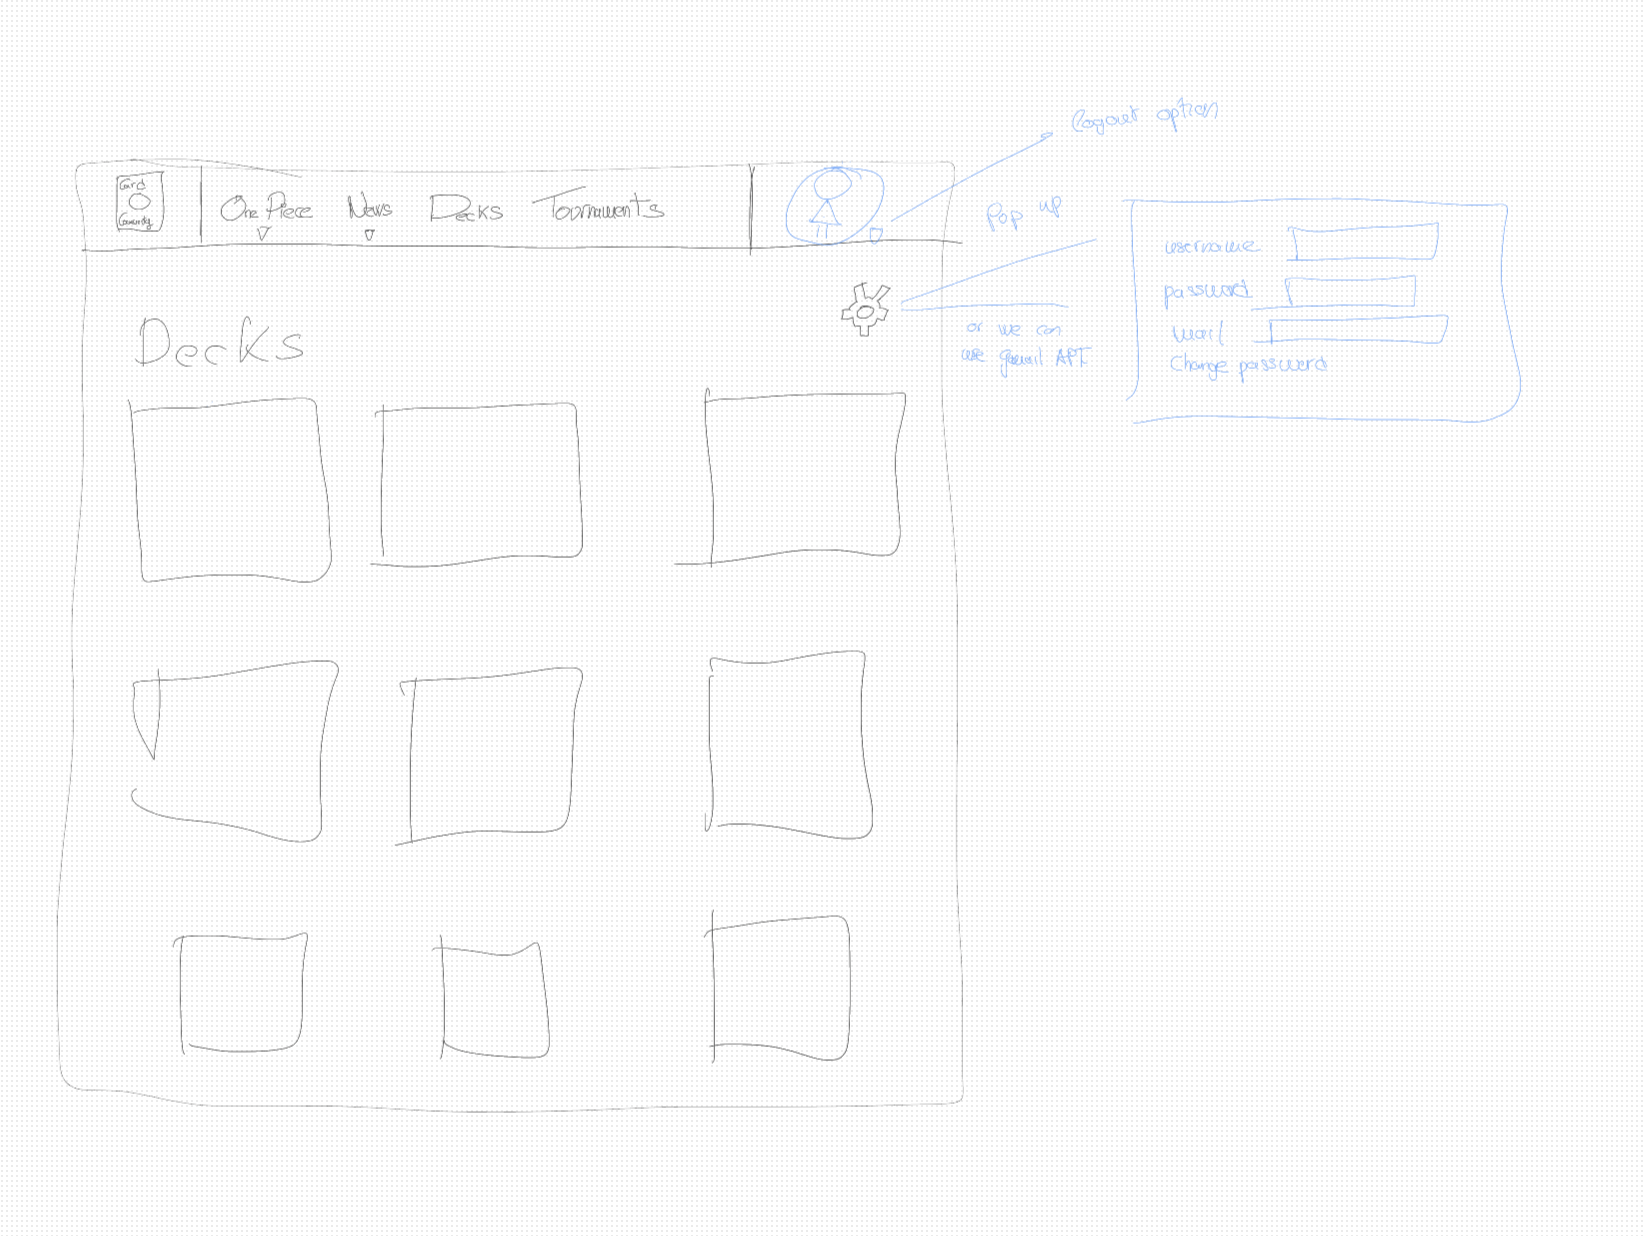
\includegraphics[width=\textwidth]{Recursos/user.png}
			\caption{Boceto de la vista del usuario donde podrá ver los mazos que ha creado y una rueda de opción realizar diferentes funciones sobre su perfil (cambiar contraseña)}
			\label{UserView}
		\end{subfigure}
	\end{figure}
	\begin{figure}[H]
		\centering
		\begin{subfigure}{0.45\textwidth}
			\centering
			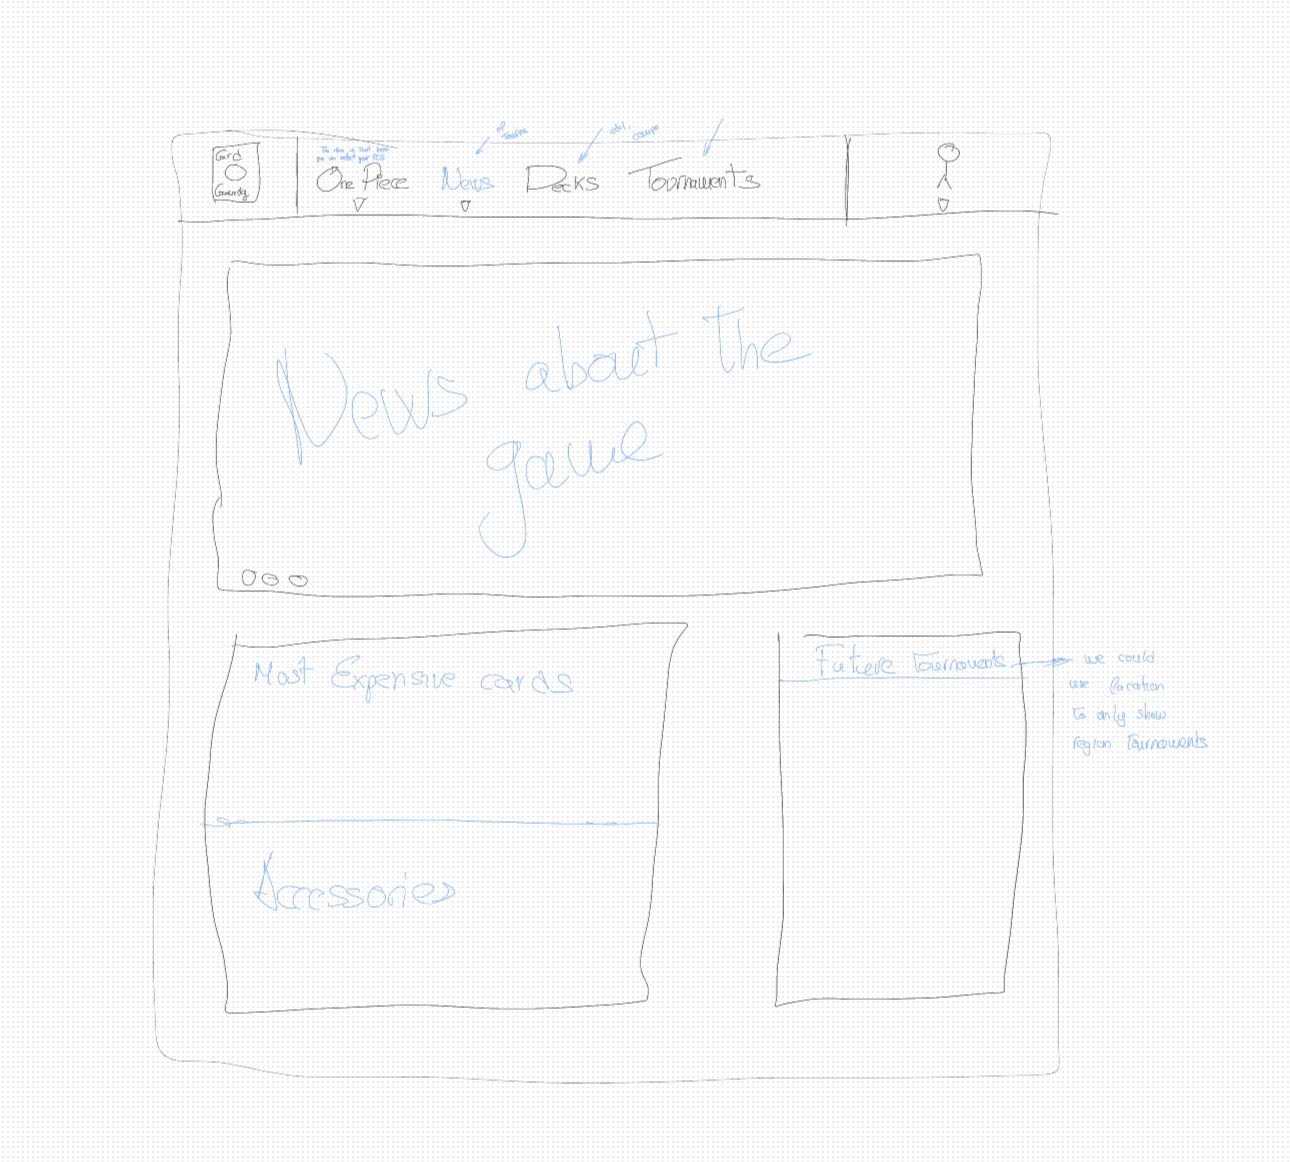
\includegraphics[width=\textwidth]{Recursos/noticias.png}
			\caption{En el apartado de noticias tendremos novedades del \textit{TCG} así como una selección de cartas más caras y de accesorios típicos para dichos juegos así como una lista de los futuros torneos.}
			\label{Noticias}
		\end{subfigure}
		\hfill 
		\begin{subfigure}{0.45\textwidth}
			\centering
			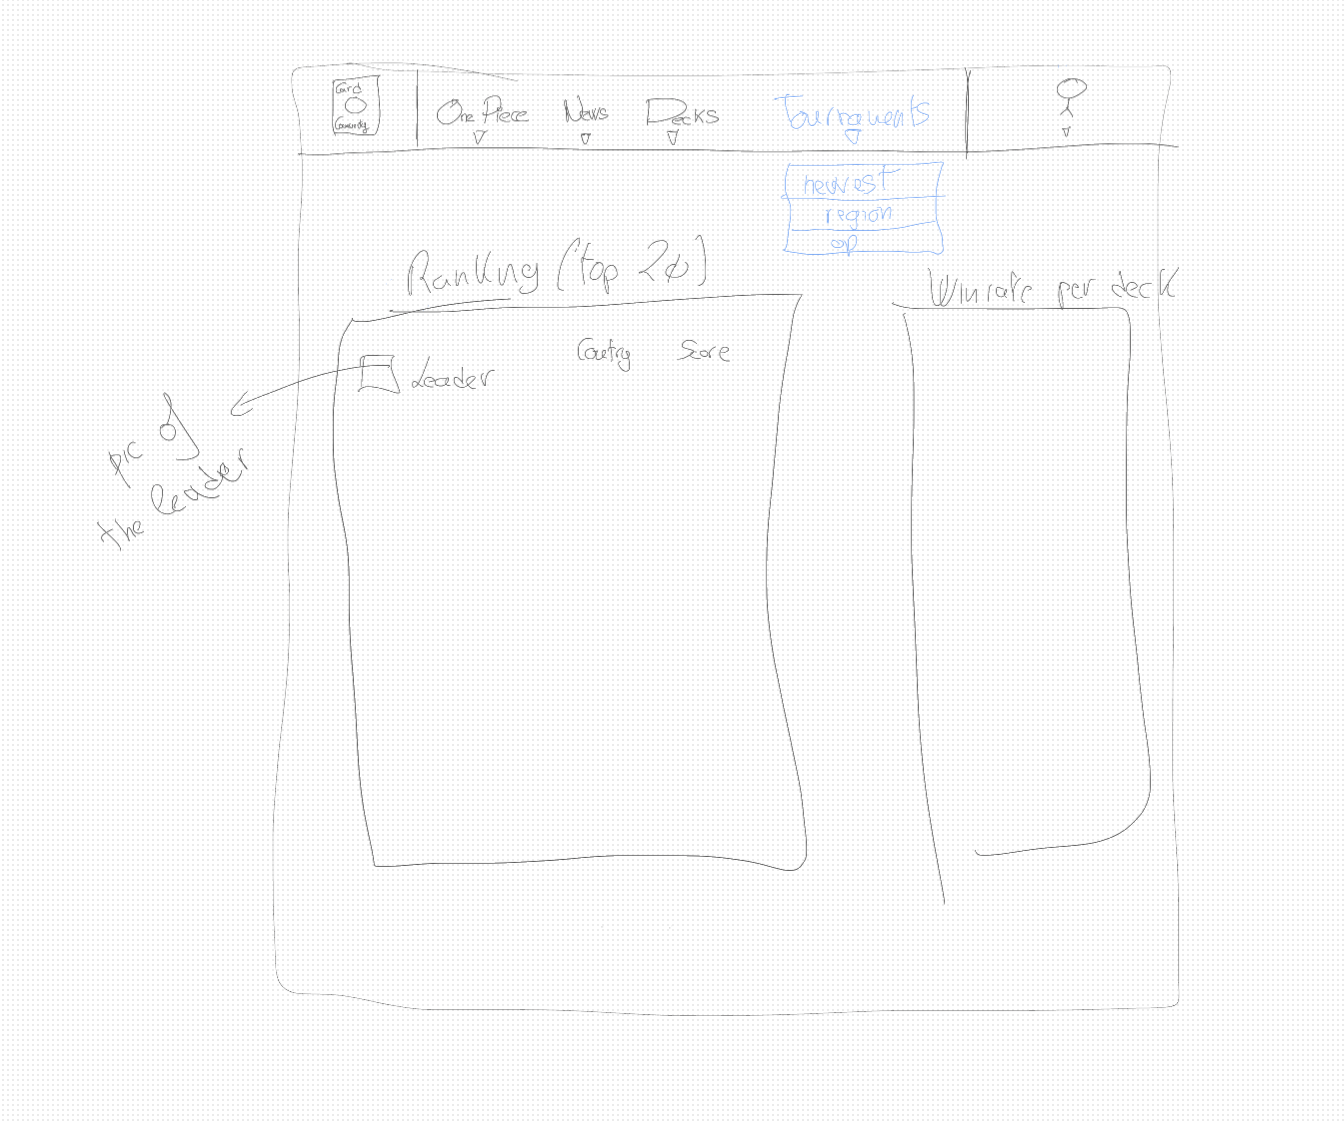
\includegraphics[width=\textwidth]{Recursos/tournaments.png}
			\caption{La pestaña de torneos con un ranking global de mazos y un \% de victoria de cada líder.}
			\label{fig:imagen_der}
		\end{subfigure}
	\end{figure}
	\begin{figure}[H]
			\centering
			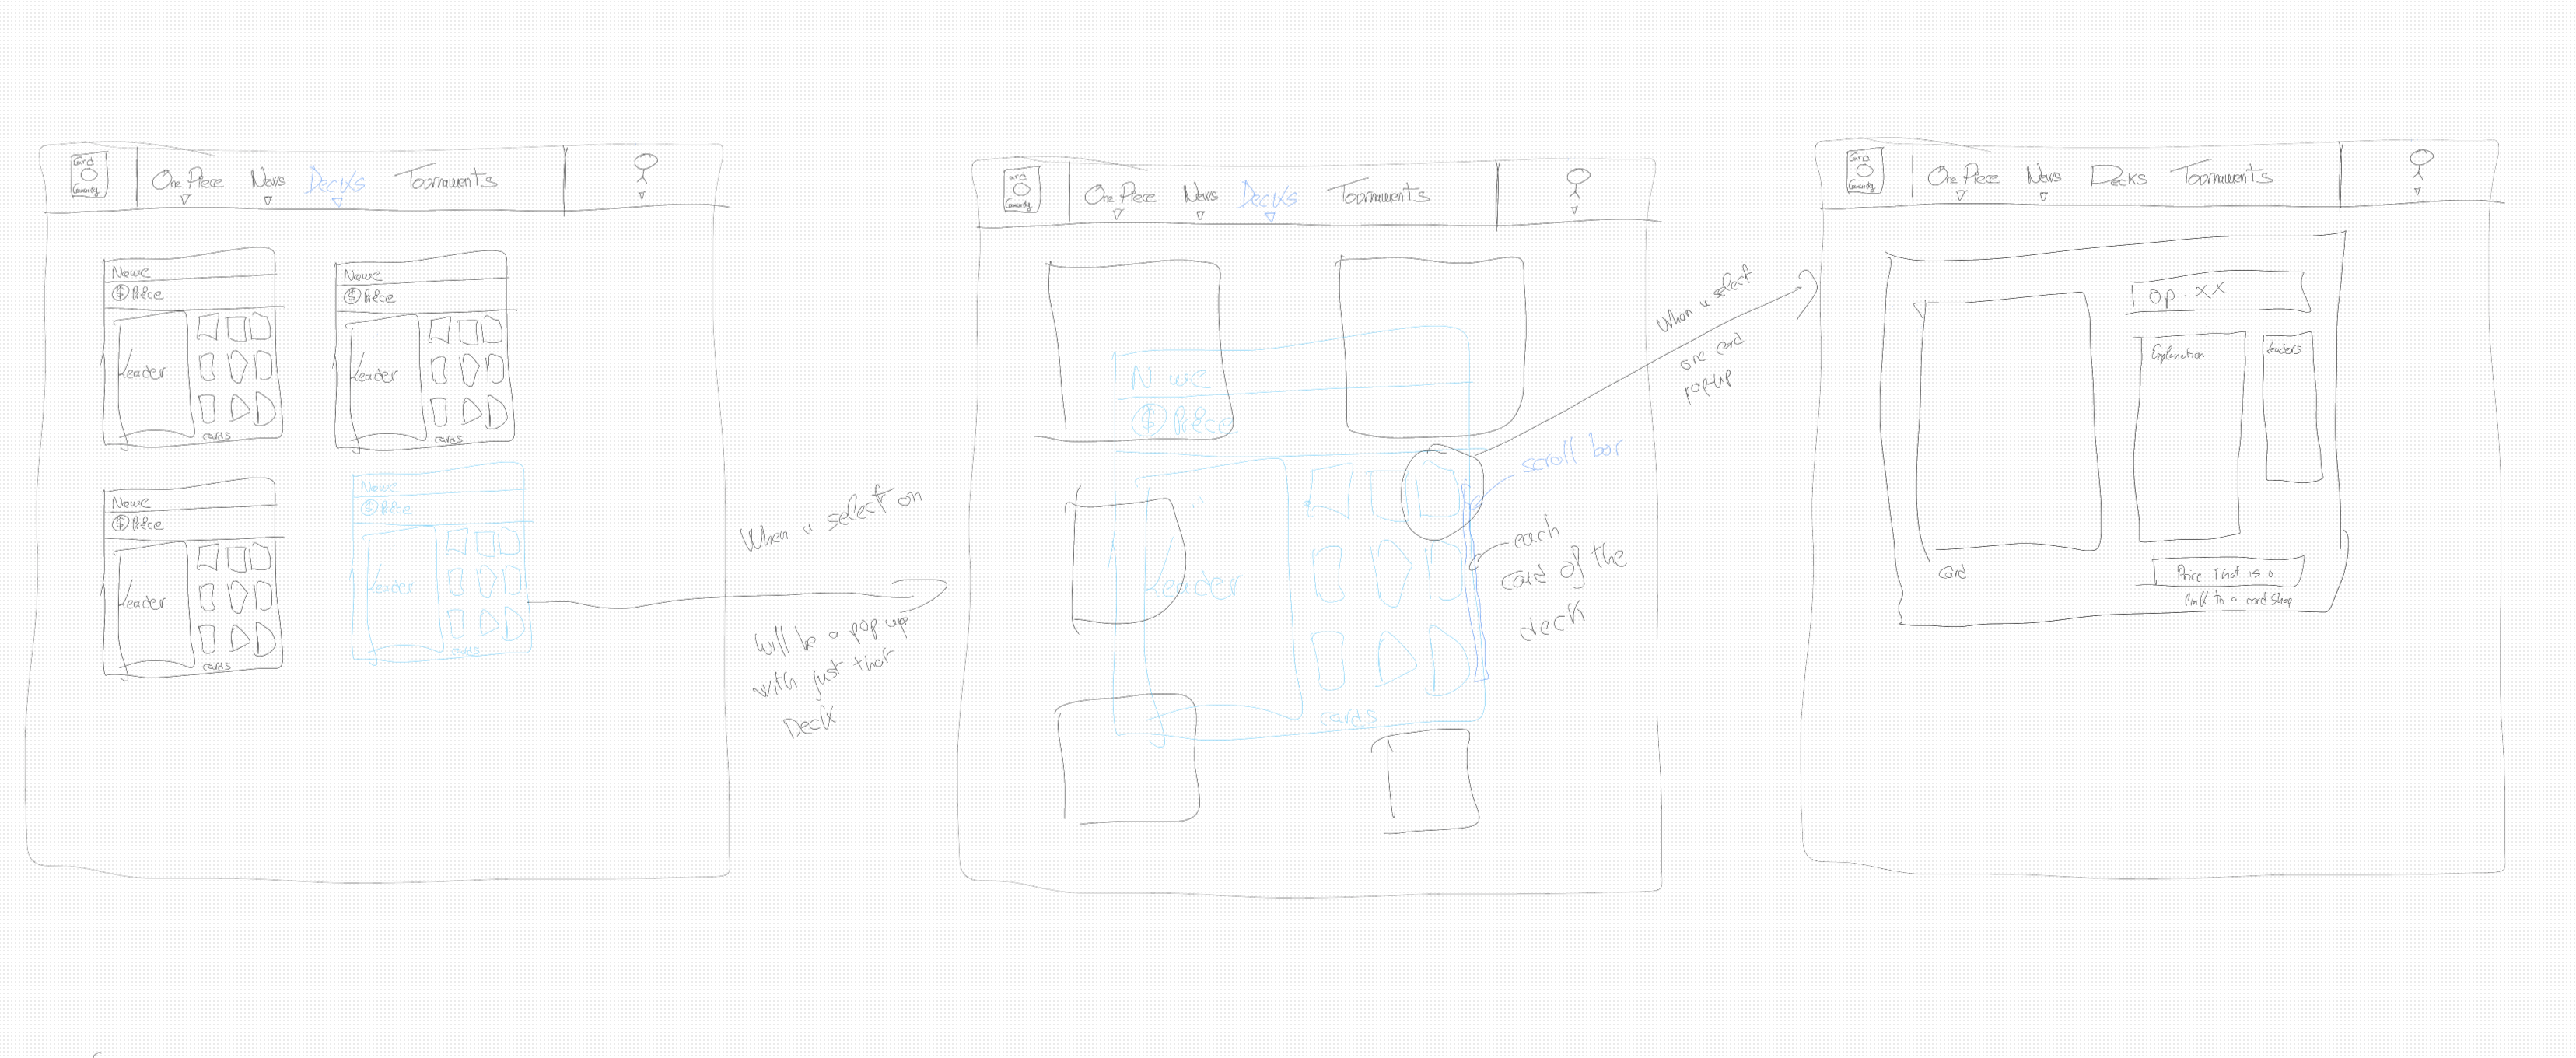
\includegraphics[width=0.85\textwidth]{Recursos/decks.png}
			\caption{En el apartado Deck, se mostraran los diferentes mazos creados por la comunidad, con la opción de seleccionar sobre ellos y poder consultar todas las cartas así como cartas en concreto de dicho mazo. Además de darle una opción a las personas con una cuenta en la web de comentar en los mazos }
	\end{figure}
	
	
	\subsection{Segunda versión del bocetaje}
	Una vez que en grupo lo revisamos, decidimos emplear una herramienta como \href{https://drive.google.com/file/d/1g8FwPydQRjYX_IET-vt37nWVM2JCpji7/view}{draw.io} para poder hacer unos bocetos más limpios y organizados (para consultar los bocetos, clickar sobre el draw.io). 
	
	Para la implementación de todas estas funcionalidades, se ha optado por organizarlas en apartados:
	\begin{itemize}
		\item \textbf{Apartado social:}
		\begin{itemize}
			\item Guias
			\item Noticias
			\item Torneos
		\end{itemize}
		
		\item \textbf{Apartado mazos:}
		\begin{itemize}
			\item Meta y estadisticas
			\item Mazos de la comunidad (con filtros de busqueda, valoraciones y comentarios)
			\item Creador de mazos
		\end{itemize}
		
		\item \textbf{Apartado cartas:}
		\begin{itemize}
			\item Listado de cartas (con filtros de busqueda, precio?, estadistica?)
		\end{itemize}
		
		\item \textbf{Apartado Usuario:}
		\begin{itemize}
			\item Iniciar sesion/Crear cuenta
			\item Información personal de la cuenta (correo, contraseña, etc)
			\item Mazos creados
			\item Mazos publicados
			\item Mazos guardados
			\item Mazos interactuados (comentario/valoracion)
		\end{itemize}
	\end{itemize}
	
	\begin{figure}[H]
		\centering
		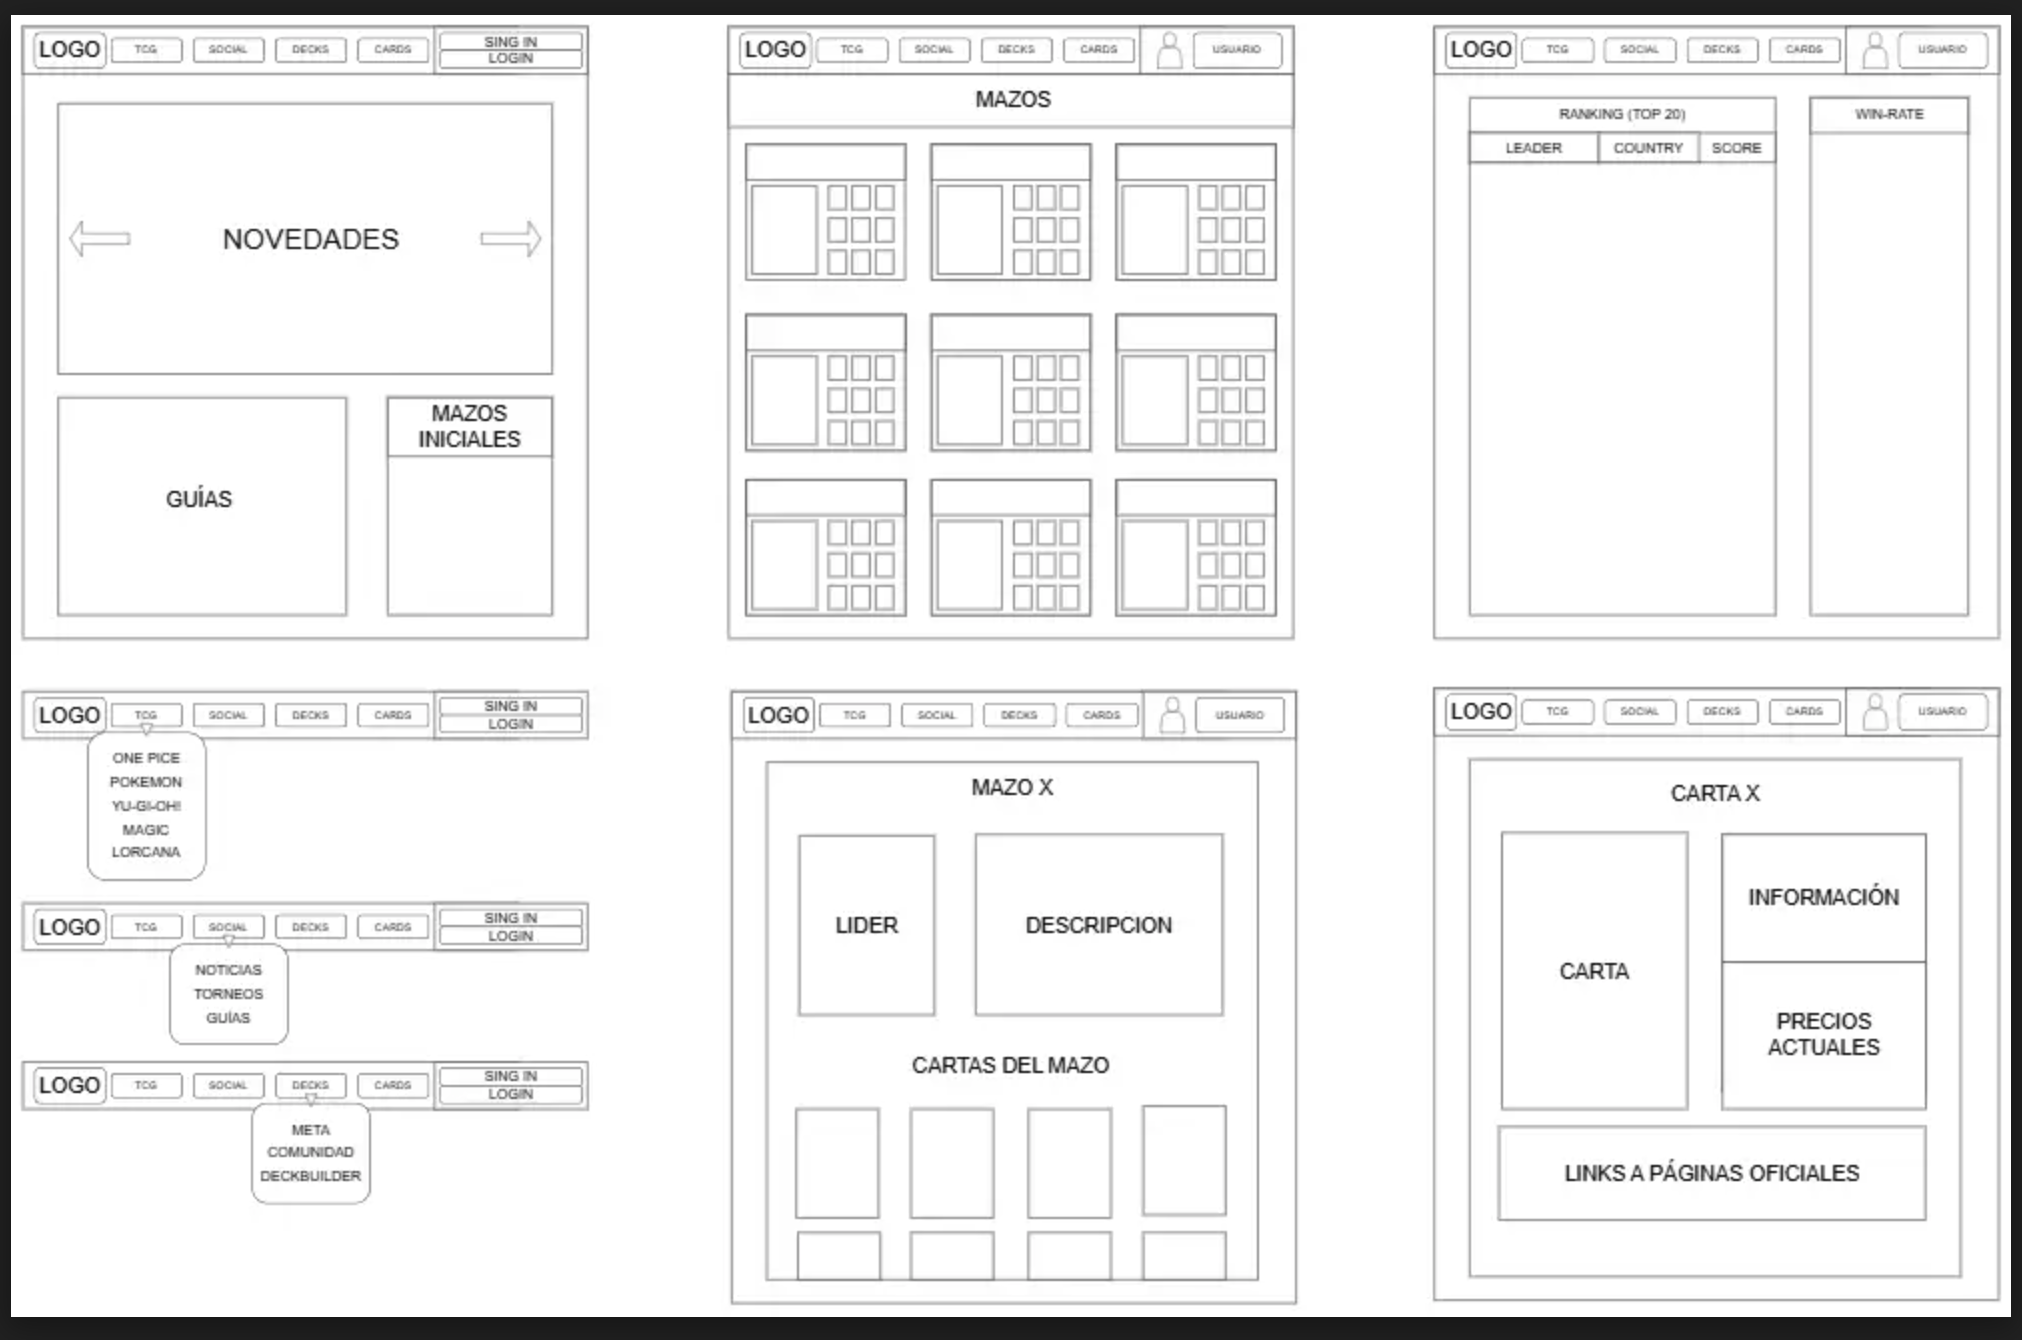
\includegraphics[width=0.85\textwidth]{Recursos/Bocetos2.png}
		\caption{\textbf{METER BOCETO ENTERO EN HORIZONTAL BIEN GUAPO}}
	\end{figure}

	\begin{figure}[H]
		\centering
		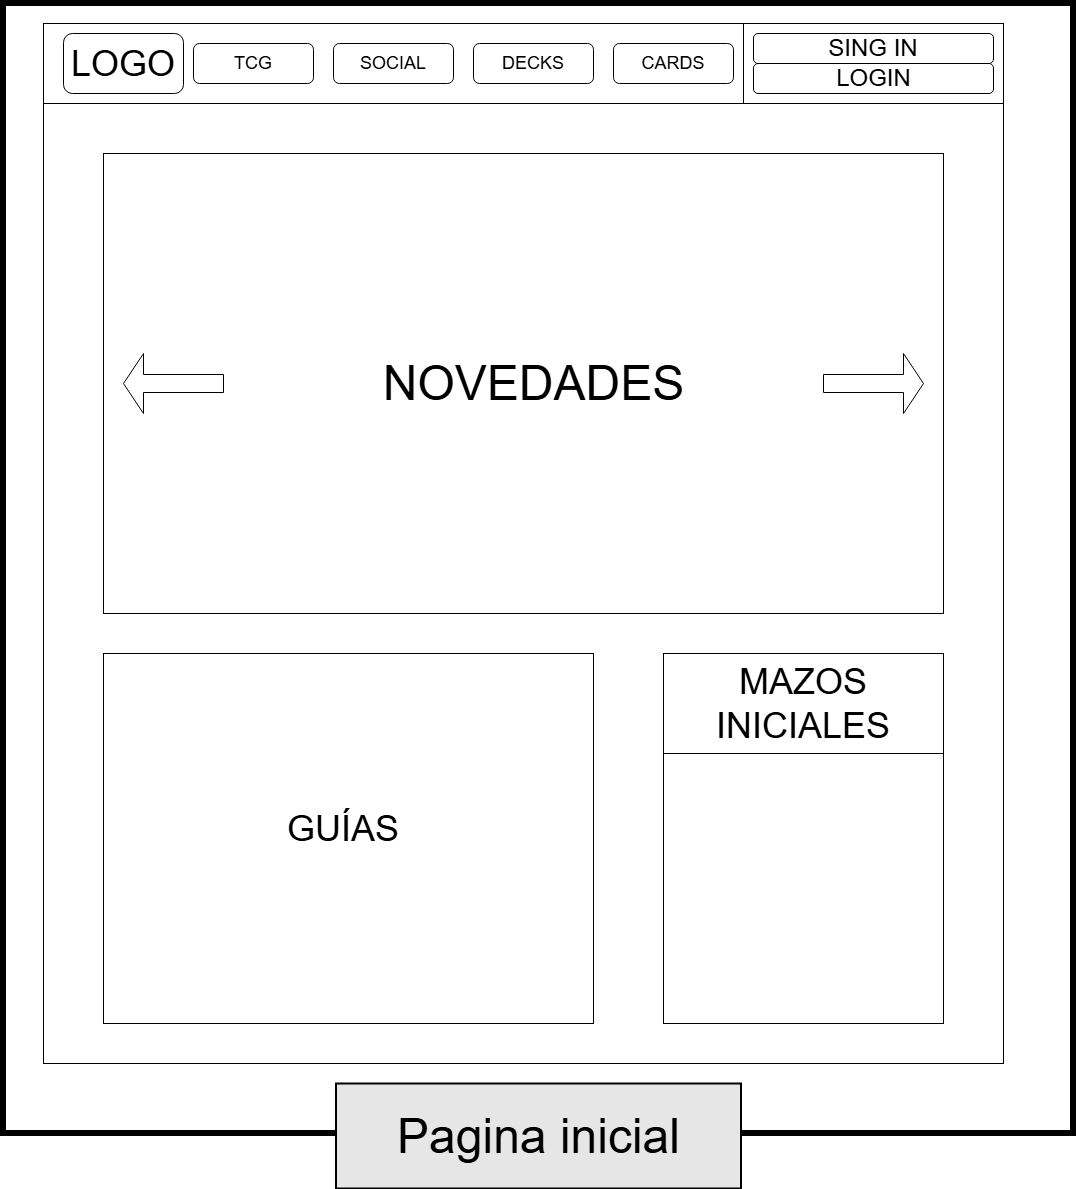
\includegraphics[width=0.85\textwidth]{Recursos/Boceto2_Inicio.png}
		\caption{\textbf{Pagina de Inicio}}
	\end{figure}
	Descripcion de pagina de Inicio
	
	\begin{figure}[H]
		\centering
		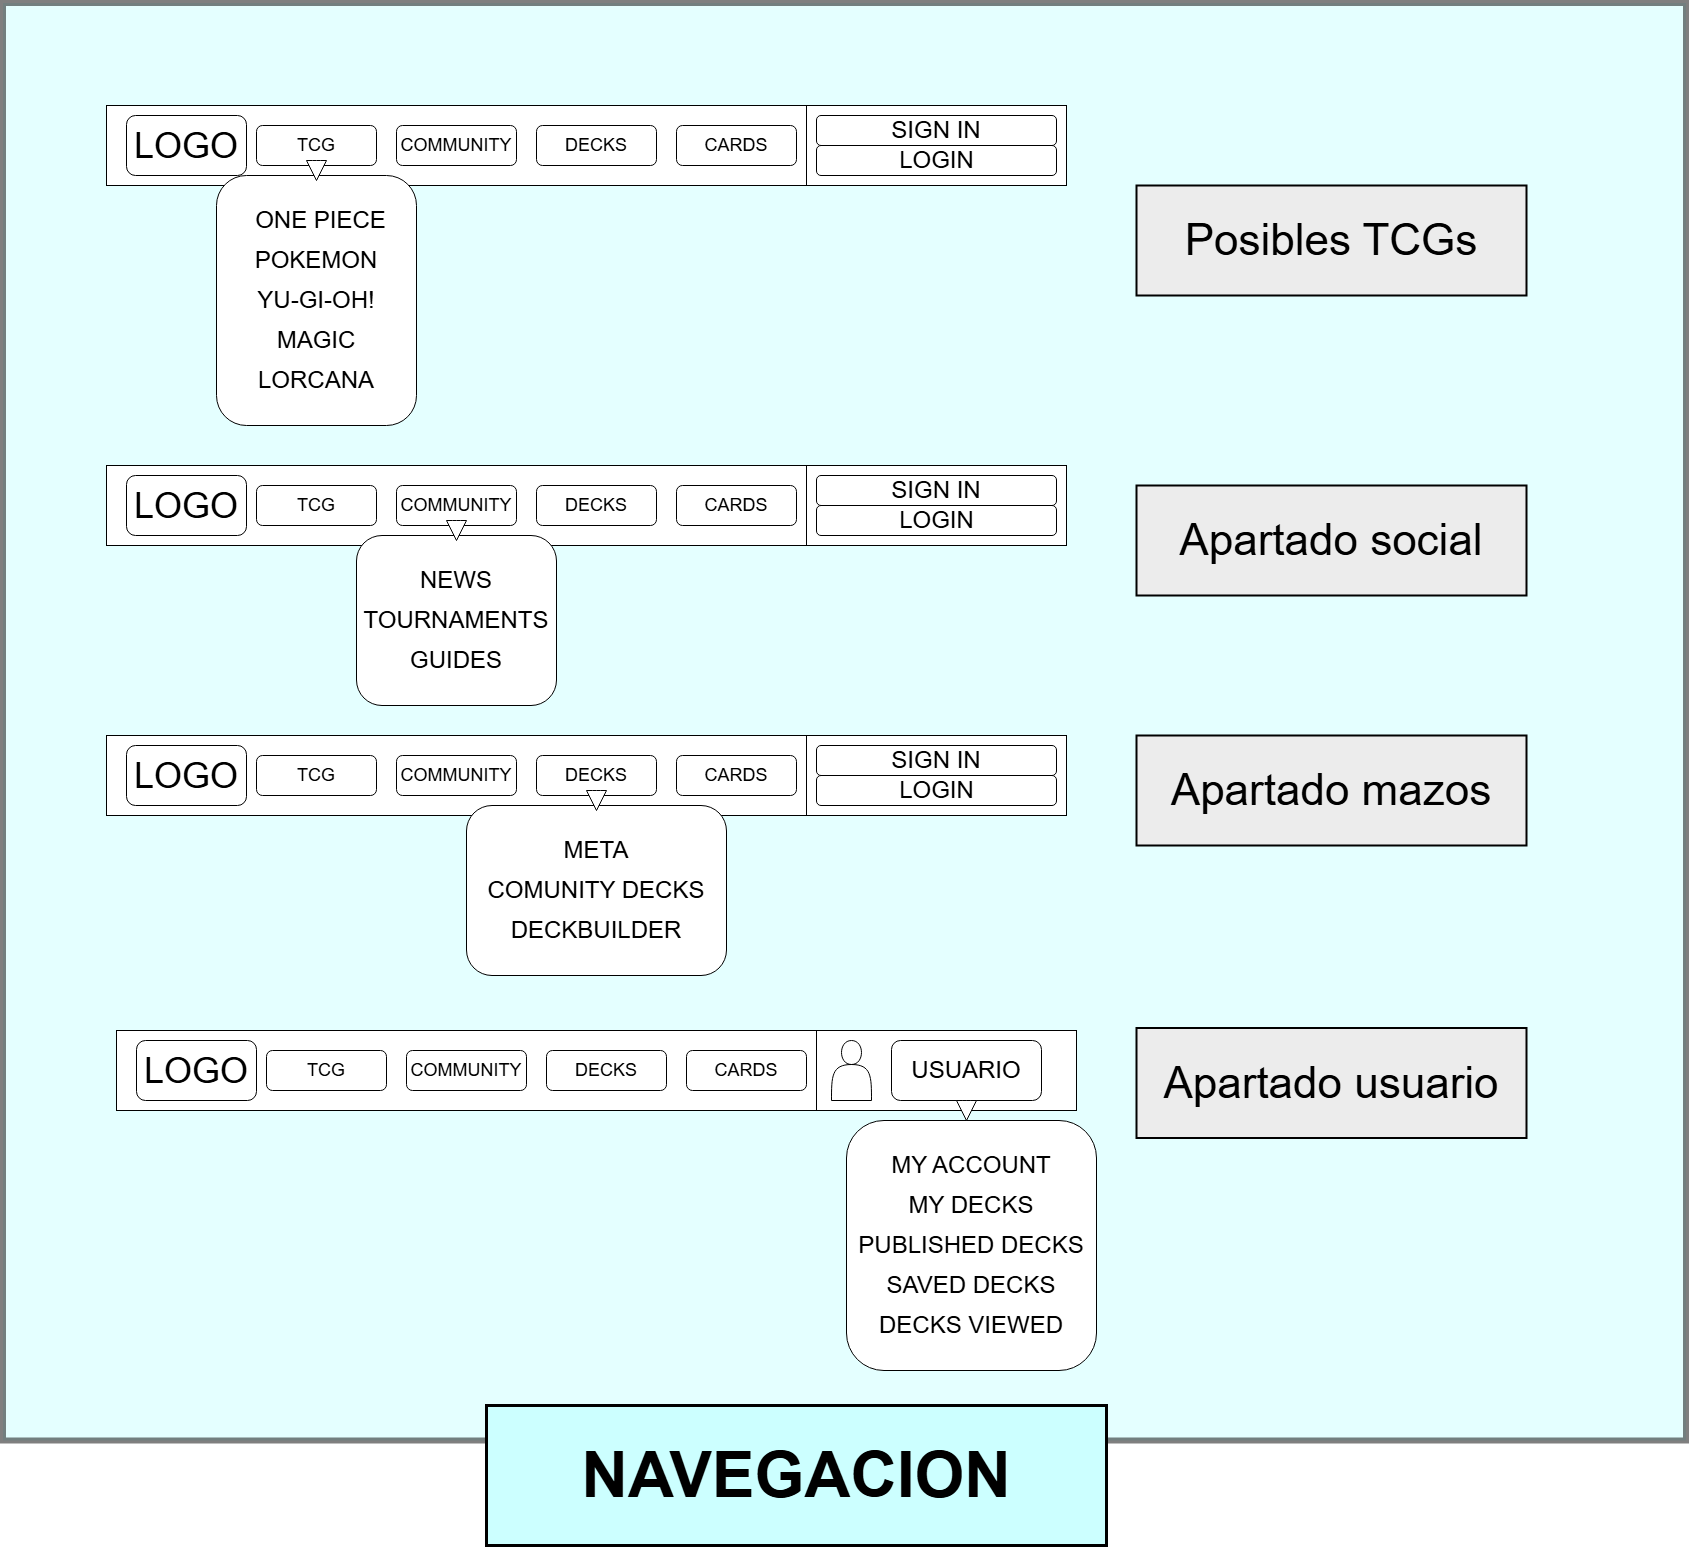
\includegraphics[width=0.85\textwidth]{Recursos/Boceto2_Navegacion.png}
		\caption{\textbf{}}
	\end{figure}
	Descripción más completa de los apartaados y como se navega por la pagina web
	
	\begin{figure}[H]
		\centering
		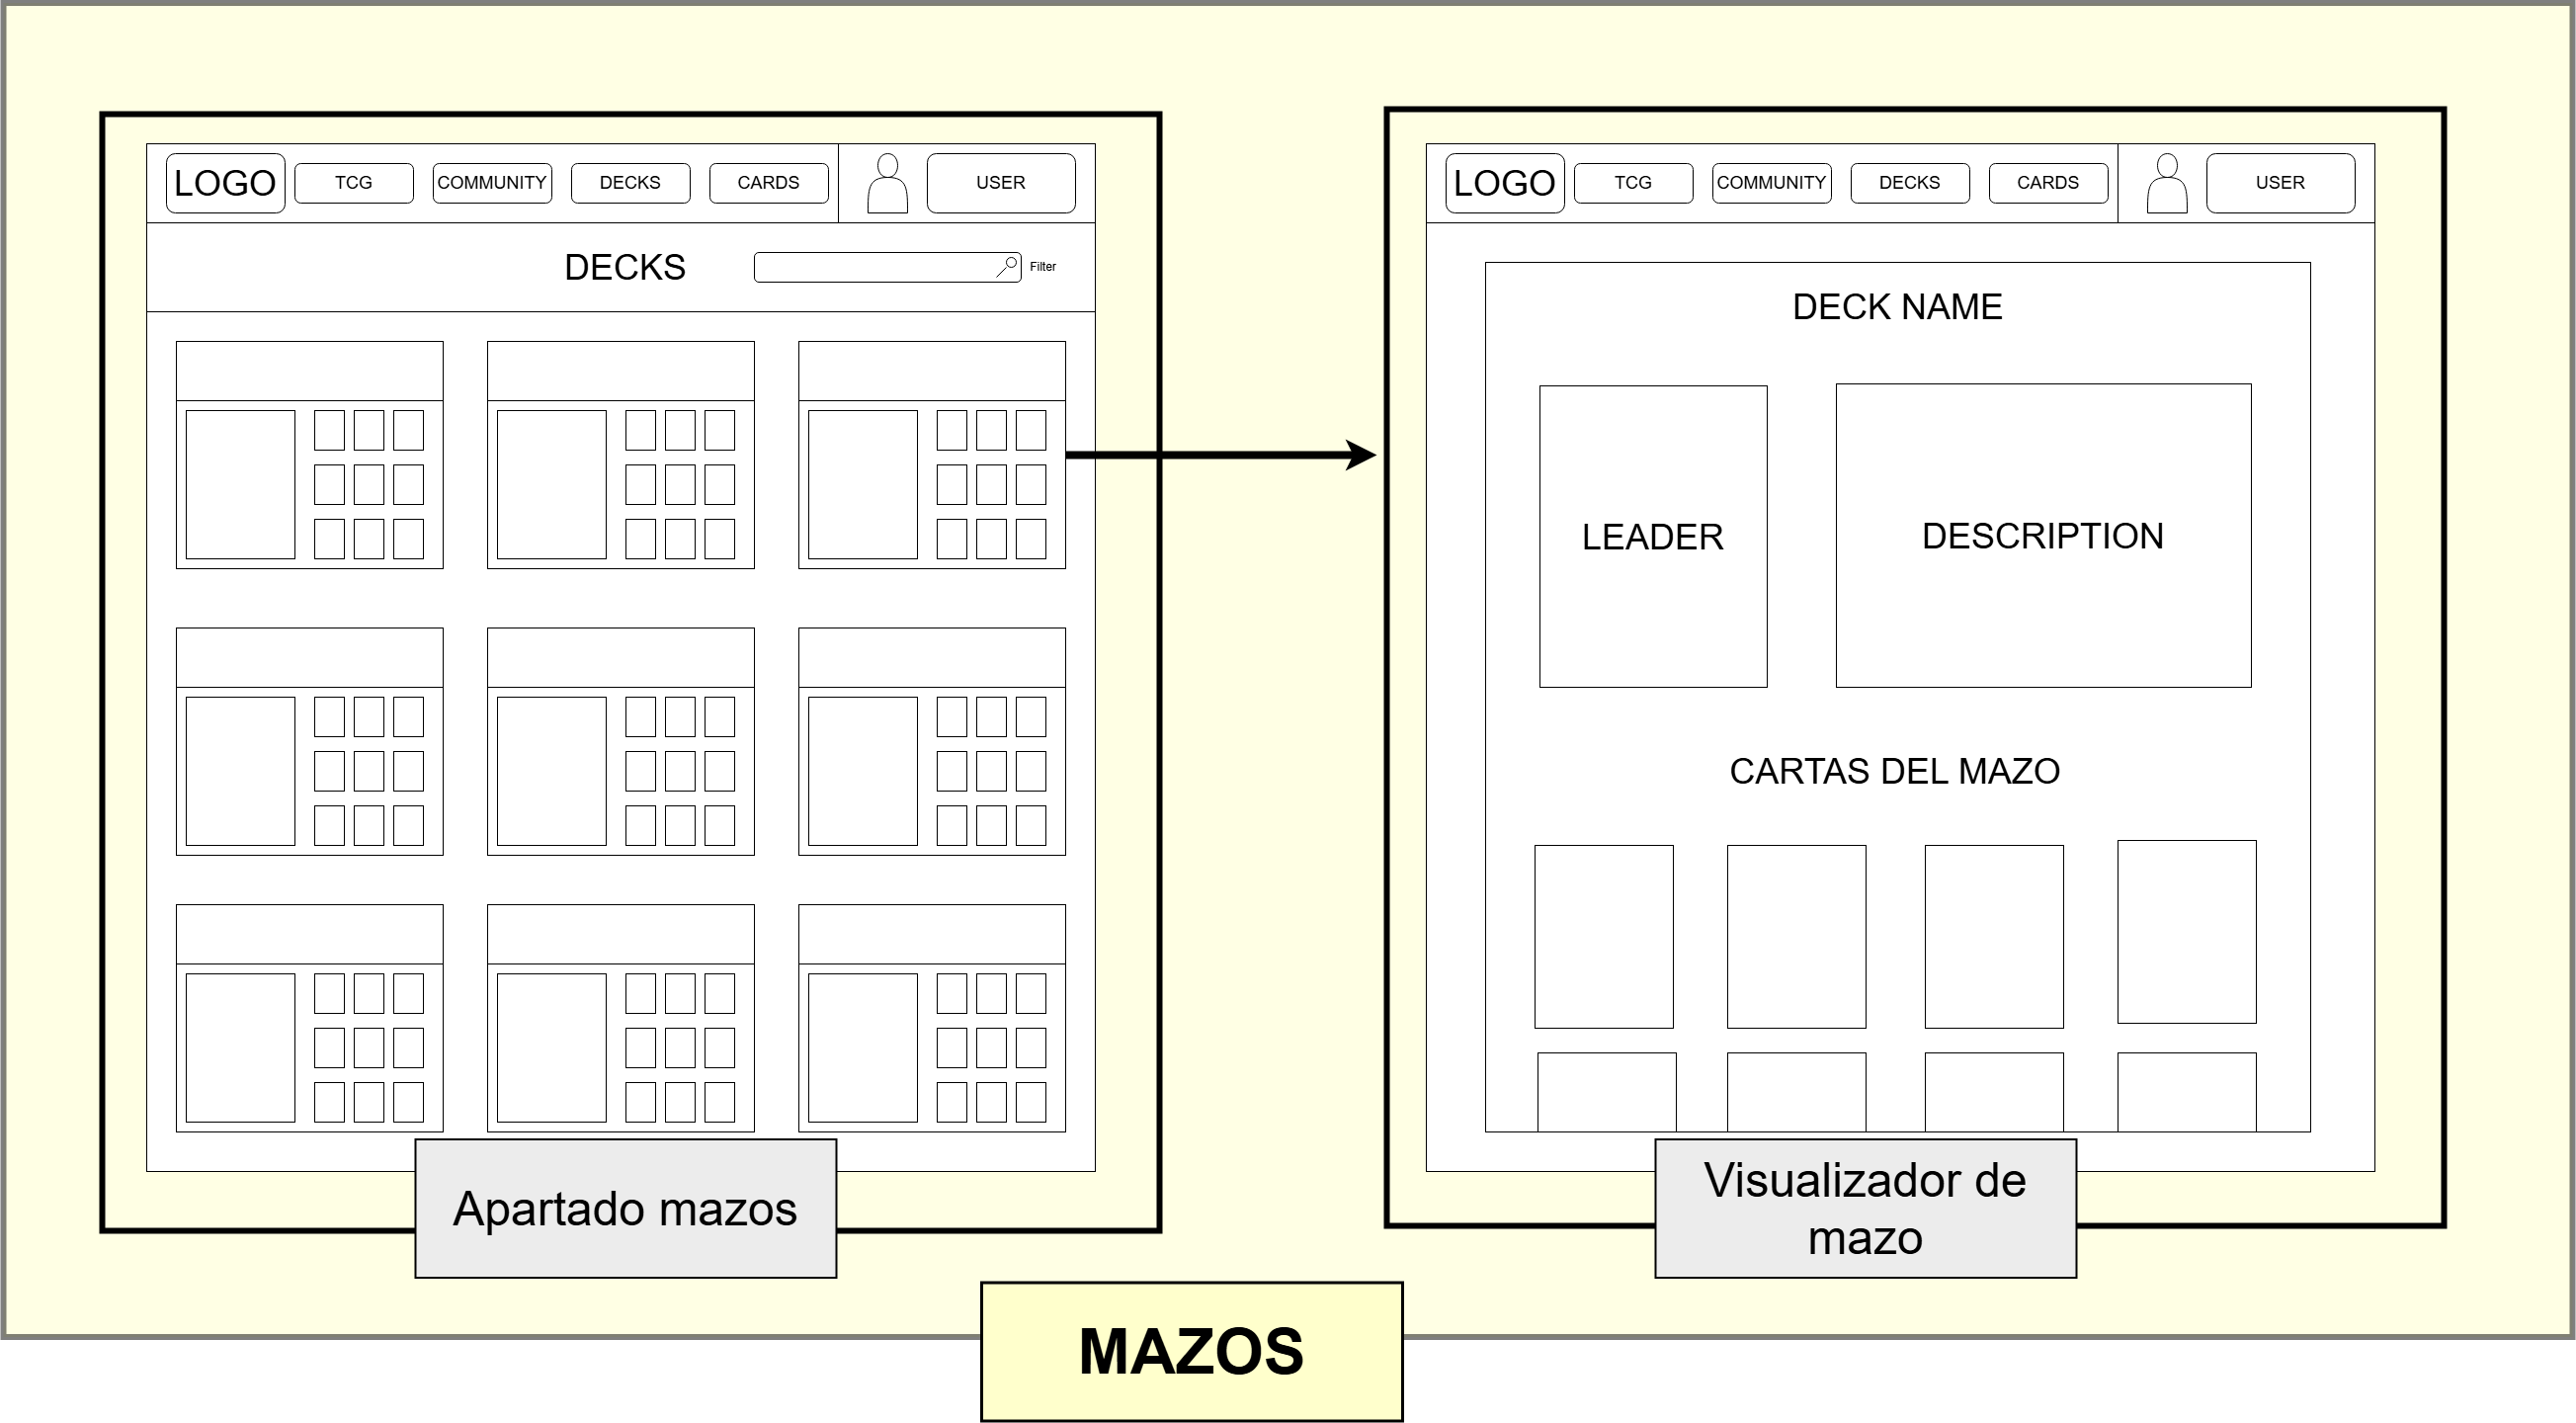
\includegraphics[width=0.85\textwidth]{Recursos/Boceto2_Mazos.png}
		\caption{\textbf{}}
	\end{figure}
	Descripcion de vision de mazos; depende de donde entres se ven mazos del meta, mazos de la comunidad, mazos tuyos, etc
	Busqueda y filtros
	Vision en profundidad del mazo seleccionado
	
	\begin{figure}[H]
		\centering
		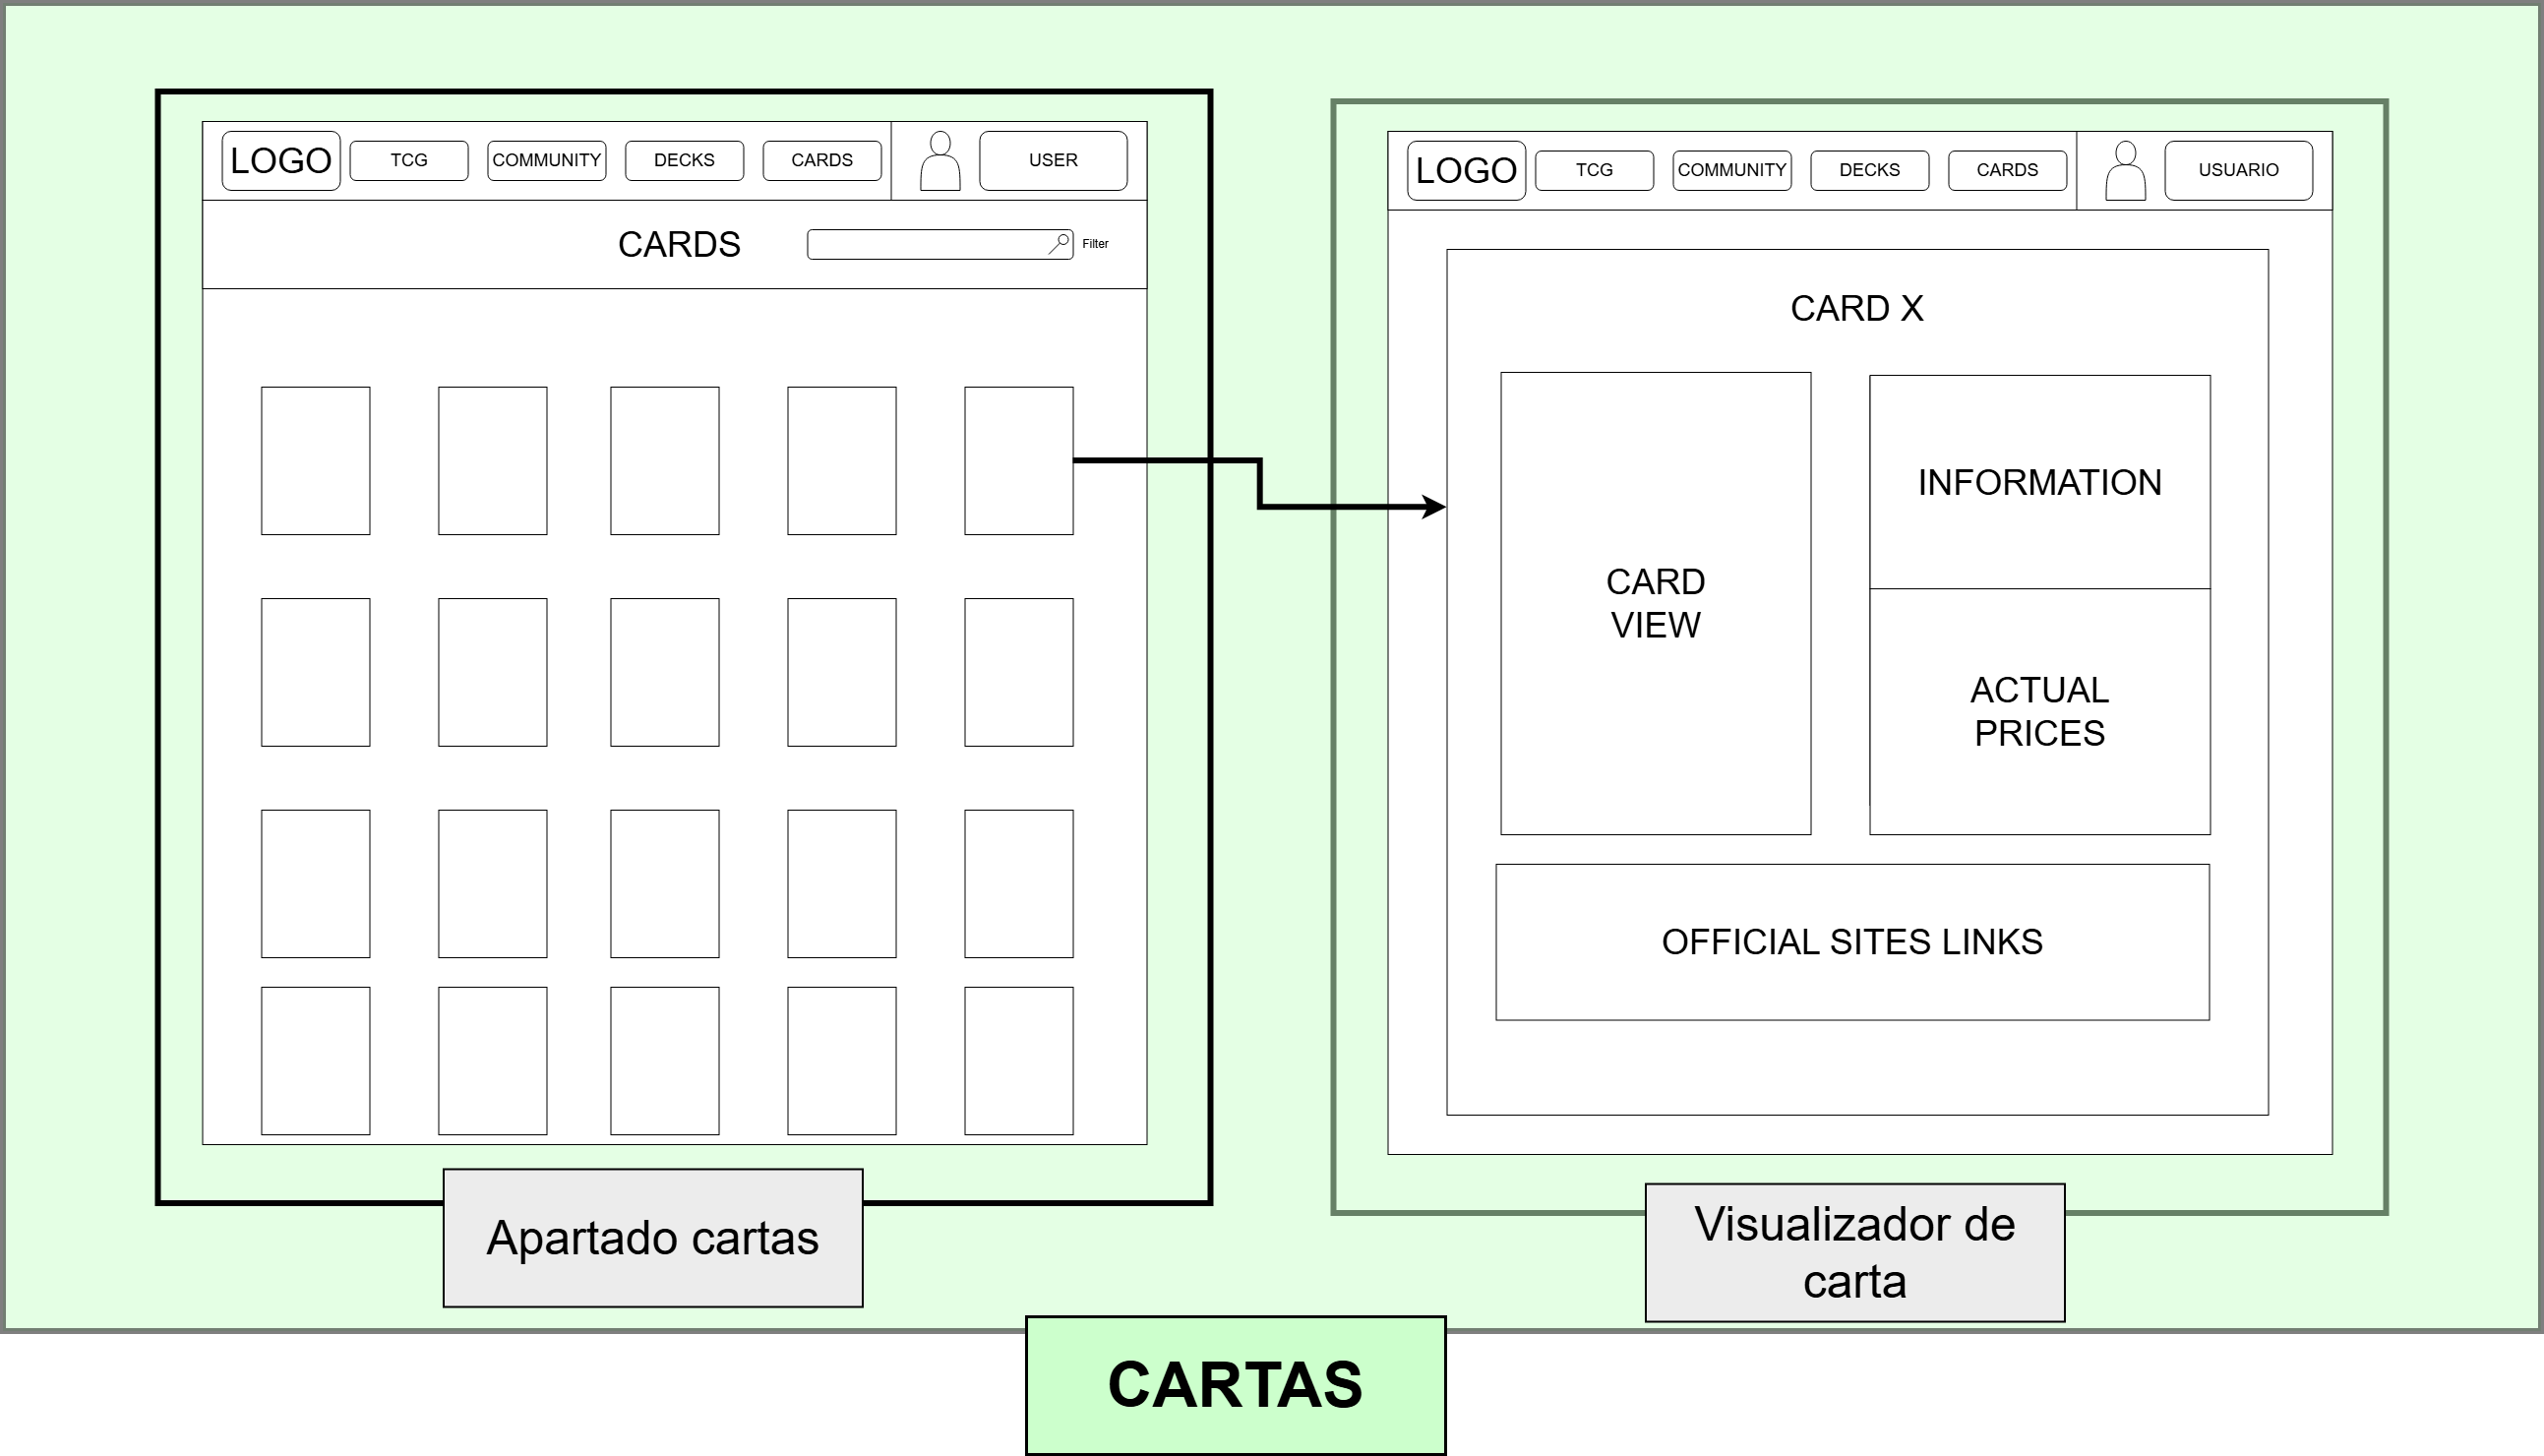
\includegraphics[width=0.85\textwidth]{Recursos/Boceto2_Cartas.png}
		\caption{\textbf{}}
	\end{figure}
	Similar a los mazos pero con las cartas, menu de todas las cartas y una vez seleccionas una, vision especifica de esa carta
	
	Faltaria creador de mazos, guias y noticias
	
	\section{Declaración de Uso de Inteligencia Artificial}
	Hemos empleado \href{https://gemini.google.com/share/938828584764}{Gemini} para dudas sobre qué se pedía en cada apartado así como de cómo realizar algunas cosas en LaTeX.
	
	
	
	%\begin{itemize}
	%   \item Herramientas utilizadas: hay que especificar qué herramientas de IA se han utilizado.
	%  \item Propósito del uso: explicar cómo se ha utilizado cada herramienta.
	% \item Alcance del uso: indicar en qué partes específicas del trabajo se ha recibido asistencia de una herramienta de IA.
	%\item Prompts utilizados: incluir los prompts, preguntas o instrucciones exactas que se han
	%introducido en la herramienta de IA.
	%\end{itemize}
	
\end{document}